\chapter{Architectures for written-text processing}

\section{Logistic Regression}

Before diving deeper into Neural Networks, it is useful to understand their littele brother: \textbf{Logistic Regression}. It can be used to classify an observation onto one of two classes (binary classification), or into one of many classes (multinomial classification). This section builds from the book Speech and Language Processing \cite{jurafskyspeech}.

Logistic Regression is a discriminative model, meaning that it models the conditional probability $P(y|x)$ directly, where $y$ is the class label and $x$ is the input feature vector. The model assumes a linear relationship between the input features and the log-odds of the class probabilities. A machine learning system for classification is based on four components:
\begin{enumerate}
    \item A \textbf{feature representation} of the input data, in the form of a vector of real-valued features $x = [x_1, x_2, \ldots, x_n]$;
    \item A classification function that computes $\hat{y}$, the estimated class, via $p(y|x)$ (see the \textbf{sigmoig} and \textbf{softmax} functions);
    \item An objective function for learning the model parameters from training data, minimizing error on the training set (in this case \textbf{cross-entropy loss function});
    \item An algorithm for optimizing the objective function, such as \textbf{gradient descent}.
\end{enumerate}

Starting from a single input observation $x$ represented as a vector of $n$ features $[x_1, x_2, \dots, x_n]$, the classifier output can be $1$ or $0$ in the \textbf{binary classification}. Logistic regression solves this task by learning, from a training set, a vector of \textbf{weights $W$} and a \textbf{bias term $b$} (which will be broadcasted to a vector in this case). The weight $w_i$ represents how important feature $x_i$ is to the classification decision. 
\[
z = \left(\sum_{i=1}^n w_i x_i\right) + b = \mathbf{w}^\top \mathbf{x} + b
\] 

To create a probability, then, we'll pass $z$ through the \textbf{sigmoid} function $\sigma(z)$, also called the \textbf{logistic function}. It has a domain of $(-\infty, +\infty)$ and a range of $(0, 1)$, making it suitable for modeling probabilities. 

\begin{minipage}{0.48\textwidth}
    \[
    \sigma(z) = \frac{1}{1 + e^{-z}}
    \]
\end{minipage}
\hfill
\begin{minipage}{0.48\textwidth}
    \begin{figure}[H]
    \centering
    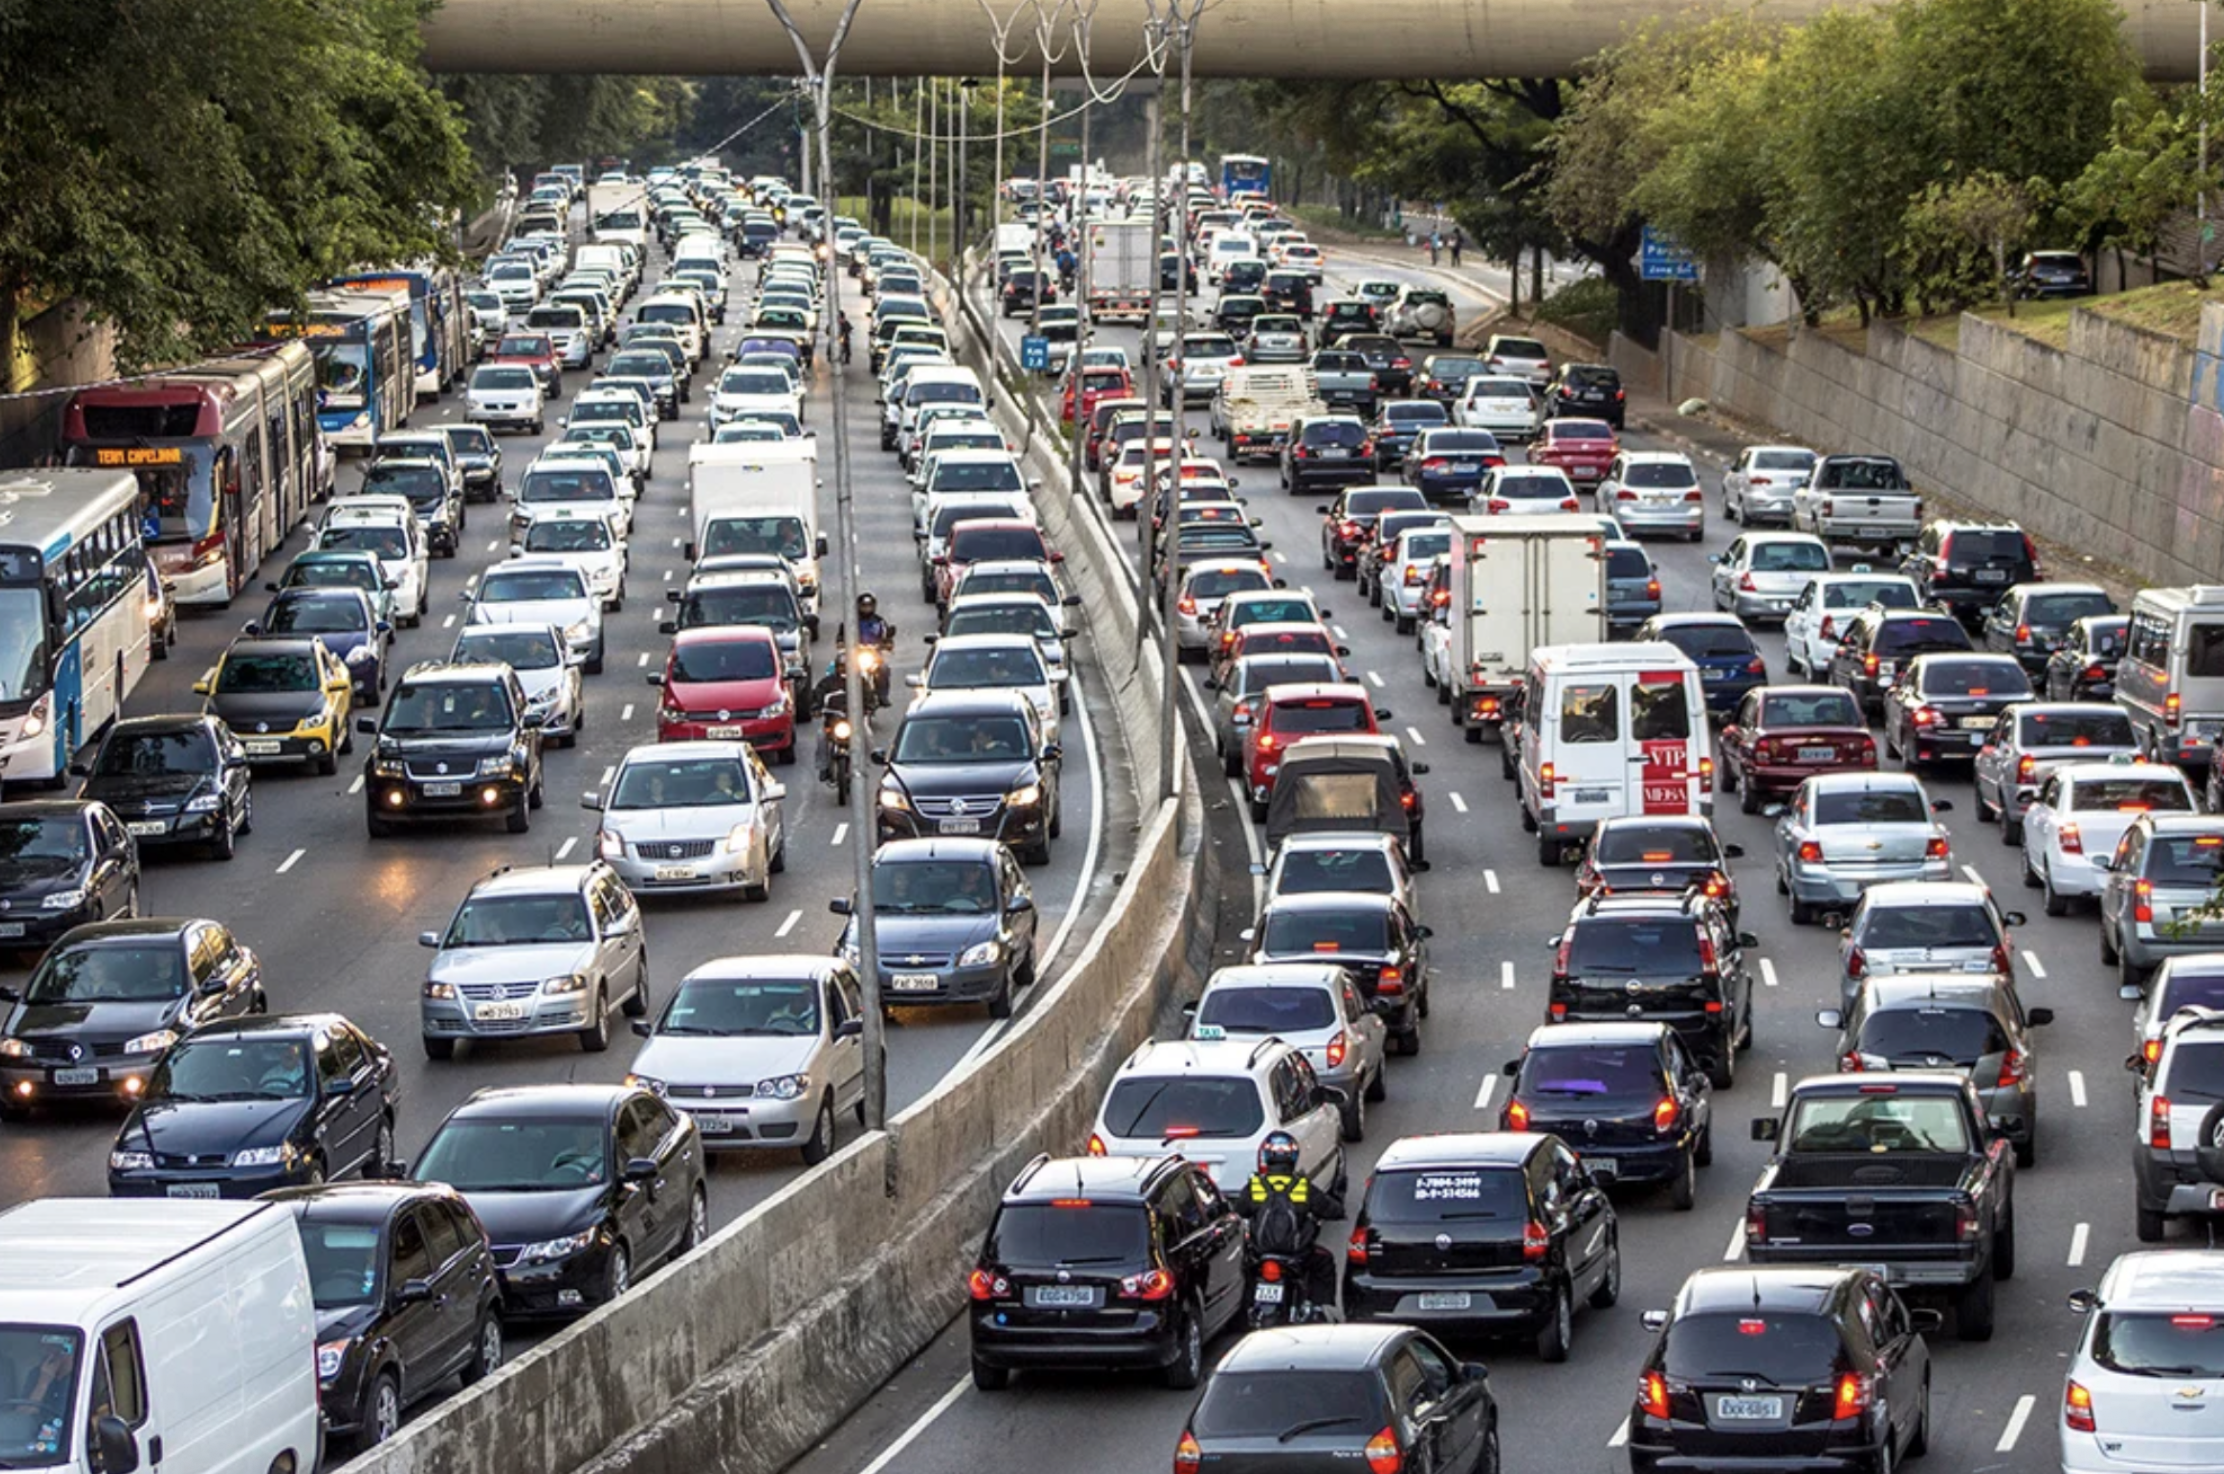
\includegraphics[width=0.6\textwidth]{assets/ch2/1.png}
\end{figure}
\end{minipage}

We can then derive the probability of class $1$ as:
\[
P(y=1|x) = \sigma(z) = \frac{1}{1 + e^{-(\mathbf{w}^\top \mathbf{x} + b)}}
\]

\begin{observationblock}
    The sigmoid function has the property
    \[
    \sigma(-z) = 1 - \sigma(z)
    \]
    which implies that
    \[
    P(y=0|x) = 1 - P(y=1|x) = \sigma(-z)
    \]
\end{observationblock}

The \textbf{decision boundary} is the value of $z$ for which we make a decision about which class to assign to a test instance $x$. Usually we set a threshold of $0.5$ for the probability of class $1$. This corresponds to $z = 0$, since $\sigma(0) = 0.5$. Therefore, if $z \geq 0$, we classify the instance as class $1$; otherwise, we classify it as class $0$.

As for now, we only consider a single example, but in practice we have to handle many of them. The most efficient approach is to use matrix multiplication to compute the outputs for all $m$ examples at once. The input data is still represented as a vector of features, but now the output must be a \textbf{one-hot vector} of $K$ values representing the classes. This way, only one of the $K$ values is $1$, indicating the correct class, while all other values are $0$. 
\[
\underbrace{\mathbf{Z}}_{(K, 1)} = \underbrace{\mathbf{W}}_{(K, n)} \underbrace{\mathbf{x}}_{(n, 1)} + \underbrace{\mathbf{b}}_{(K, 1)}
\]

Moreover, the \textbf{softmax} function is used in this case. It is a generalization of the sigmoid function for multi-class classification problems, where there are more than two classes. The softmax function takes a vector of real-valued scores (logits) and converts them into a probability distribution over multiple classes. Given a vector of logits $\mathbf{z} = [z_1, z_2, \ldots, z_k]$, the softmax function computes the probability of each class $i$ as follows:
\[
P(y=i|\mathbf{z}) = \frac{e^{z_i}}{\sum_{j=1}^k e^{z_j}}
\]

Applying the softmax function to the logistic regression model, we have to separate weight vectors $\mathbf{w}_i$ and bias $b_i$ for each of the $K$ classes. 
\[
p(y_i|\mathbf{x}) = \frac{e^{\mathbf{w}_i^\top \mathbf{x} + b_i}}{\sum_{j=1}^K e^{\mathbf{w}_j^\top \mathbf{x} + b_j}}  
\]
where $\mathbf{w}$ has shape $[n, K]$ and $\mathbf{b}$ has shape $[K, 1]$.

\[
\underbrace{\hat{y}}_{(K, 1)} = softmax(\underbrace{\mathbf{W}}_{(K, n)} \underbrace{\mathbf{x}}_{(n, 1)} + \underbrace{\mathbf{b}}_{(K, 1)})
\]

\subsection{Cross-entropy Loss Function}

We now need a loss function that expresses, for an observation $x$, how close the classifier output $\hat{y}$ is to the correct output $y$. We do this via a loss function that prefers the correct class labels of the training examples to be \textit{more likely}. We therefore choose the parameters $\mathbf{W}$ and $\mathbf{b}$ that maximize the likelihood of the correct class labels in the training data. This is equivalent to minimizing the \textbf{cross-entropy loss function}, which is defined as follows for a single training example:
\[
L(\hat{y}, y) = - \log p(y|x) = -\left[y\log\hat{y} + (1-y)\log(1-\hat{y})\right]
\]

\begin{observationblock}[Cross-entropy Loss = Negative Log-Likelihood]
    The information an event $x$ carries is defined as $I(x) = -\log P(x)$. The cross-entropy between two probability distributions $p$ and $q$ over the same set of events measures the average number of bits needed to identify an event drawn from the set, if a coding scheme used for the set is optimized for an estimated probability distribution $q$, rather than the true distribution $p$. It is defined as:
    \[
    H(p, q) = - \sum_x p(x) \log q(x)
    \]
    We can notice that the cross-entropy loss function is equivalent to the negative log-likelihood of the correct class label (look at the binary classification to understand better).
\end{observationblock}

The cross-entropy loss function can be written also as:
\[
L(\hat{y}, y) = - \sum_{i=1}^K y_i \log \hat{y}_i
\]

We now need an algorithm to minimize the loss function over the training set. A common choice is \textbf{gradient descent}, which iteratively updates the model parameters in the direction of the negative gradient of the loss function with respect to the parameters. The update rule for the weights and bias is as follows:
\[
\mathbf{W} := \mathbf{W} - \eta \nabla_{\mathbf{W}} L(\hat{y}, y)
\]
where $\eta$ is the learning rate, a hyperparameter that controls the step size of each update.

\begin{warningblock}
    To use the gradient descent algorithm, we need to be able to compute the gradient of the loss function with respect to the model parameters. This is done using the \textbf{backpropagation} algorithm, which efficiently computes the gradients by applying the chain rule of calculus, but also introduces the need to have proper differentiable functions in the model. 
\end{warningblock}

The gradient descent algorithm can be applied in two main ways: \textbf{batch gradient descent} and \textbf{stochastic gradient descent (SGD)}. In batch gradient descent, the gradients are computed using the entire training set, while in SGD, the gradients are computed using a single training example at a time. A compromise between these two approaches is \textbf{mini-batch gradient descent}, where the gradients are computed using a small subset of the training set (mini-batch) at each iteration.

It's now time to generalize the loss function from 2 to $K$ classes. We represent both $y$ and $\hat{y}$ as vectors, and the loss function is the sum of the logs of th $K$ output classes, each weighted by their probability $y_i$:

\begin{align*}
L(\hat{y}, y) &= - \sum_{i=1}^K y_i \log \hat{y}_i \\
&= - \log \hat{\mathbf{y_c}} \quad \text{(where } c \text{ is the correct class)} \\
&= -\log \frac{\exp{\mathbf{w}_c \mathbf{x} + b_c}}{\sum_{j=1}^K \exp{\mathbf{w}_j \mathbf{x} + b_j}} \\
\end{align*}

Moreover, we can derive the partial derivative of the loss with respect to $\mathbf{w}_{k,i}$ as:
\[
\frac{\partial L}{\partial \mathbf{w}_{k,i}} = (\hat{y}_i - y_i) x_k
\]

\begin{advancedblock}[Deriving the Gradient Equation]
    The \textbf{chain rule} is a fundamental rule in calculus that allows us to compute the derivative of a composite function. It states that if we have two functions $f(g(x))$, then the derivative of the composite function with respect to $x$ is given by:
    \[
    \frac{d}{dx} f(g(x)) = f'(g(x)) \cdot g'(x)
    \]
    Using the chain rule, we can derive the partial derivative of the loss function with respect to $\mathbf{w}_{k,i}$ as follows:
    \begin{align*}
    \frac{\partial L}{\partial \mathbf{w}_{k,i}} &= - \frac{\partial}{\partial \mathbf{w}_{k,i}} \log \hat{y}_c \\
    &= - \frac{1}{\hat{y}_c} \cdot \frac{\partial \hat{y}_c}{\partial \mathbf{w}_{k,i}} \\
    &= - \frac{1}{\hat{y}_c} \cdot \frac{\partial}{\partial \mathbf{w}_{k,i}} \left( \frac{e^{\mathbf{w}_c \mathbf{x} + b_c}}{\sum_{j=1}^K e^{\mathbf{w}_j \mathbf{x} + b_j}} \right) \\
    &= - \frac{1}{\hat{y}_c} \cdot \left( \frac{e^{\mathbf{w}_c \mathbf{x} + b_c} x_k (\delta_{i,c} - \hat{y}_i)}{\sum_{j=1}^K e^{\mathbf{w}_j \mathbf{x} + b_j}} \right) \\
    &= - (1) x_k (\delta_{i,c} - \hat{y}_i) \\
    &= (\hat{y}_i - y_i) x_k
    \end{align*}
    where $\delta_{i,c}$ is the Kronecker delta, which is $1$ if $i = c$ and $0$ otherwise.
\end{advancedblock}

\newpage
\section{Embeddings}

Vector semantics is the standard way to represent word meaning in NLP. It derives from two ideas: using a point in a 3D space to represent the connotation of a word and defining the meaning of a word by its \textbf{distribution} in language use, considering the neighborhood of words that tend to occur near it. 

\begin{definitionblock}[Embeddings]
    An \textbf{embedding} is simply a multidimensional vector to represent words or other discrete items. The idea is to map each word to a point in a continuous vector space, where semantically similar words are mapped to nearby points. 
\end{definitionblock}

They are \textbf{dense} vectors, meaning that the number of dimensions is much lower than the vocabulary size $|V|$, and these dimensions don't have a clear interpretation. Having dense vectors instead of sparse ones helps in different tasks, since we have to learn much less weights. Here we will dive deeper into one model: the \textbf{skip-gram with negative sampling (SGNS)}, usually referred to also as Word2Vec.

\begin{observationblock}[Cosine Similarity]
    To measure similarity between two target words $v$ and $w$, we need a metric that takes two vectors (of the same dimensionality) and gives a measure of similarity. We consider here the \textbf{cosine similarity}, which measures the angle between the two vectrs. It is based on the dot product, in fact it is a \textbf{normalized dot product}, corrected since the normal one favors long vectors ($|\mathbf{v}|$):
    \[
    cosine(\mathbf{v}, \mathbf{w}) = \frac{\mathbf{v}\cdot\mathbf{w}}{|\mathbf{v}||\mathbf{w}|} = \frac{\sum_{i=1}^N v_i w_i}{\sqrt{\sum_{i=1}^N v_i^2}\sqrt{\sum_{i=1}^N w_i^2}}
    \] 
    The cosine value ranges from 1 for vectors pointing in the same direction, through 0 for orthogolan vectors, to -1 for vectors pointing in opposite directions. 
\end{observationblock}

Word2Vec embeddings are \textbf{static embeddings}, meaning that the method learns one fixed embedding for each word in the vocaboulary, contrary to the \textbf{contextual embeddings} that will be later explained. Its intuition is to train a classifier on a binary prediction task ("Is word $w$ likely to show up near word $c$?") and then use the learned weights (initialized randomly) as embeddings. It seems like a cycle, but remember that the embeddings are the weights and the whole procedure of learning them is the algorithm. An important consideration is that we can apply \textbf{self-supervision} in this case, since we can check in an online way if our prediction is corrext just by using running text.

Given a text, we want to train a classifier such that, given a tuple $(w,c)$ of a target word $w$ paired with a candidate context word $c$, it will return the probability that $c$ is a real context word. 

\[
P(+|w,c)
\]

To compute this probability, we use embedding similarity: a word is likely to occur near the target if its embeddings (weights) are simiar to the ones of the target. We then consider the \textbf{dot product}:

\[
Similarity(w,c) \approx \mathbf{c} \cdot \mathbf{w}
\]

To have a probability, we then use the \textbf{sigmoid} function:

\[
P(+|w,c) = \sigma(\mathbf{c}\cdot\mathbf{w}) = \frac{1}{1 + e^{-\mathbf{c}\cdot\mathbf{w}}}
\]

Since we also need the total probability of all the cases to be 1, and simplifying using the independence assumption, we have that:

\[
P(+|w,c_{1:L}) = \prod_{i=1}^L P(+|w,c_i) = \prod_{i=1}^L \sigma(\mathbf{c}_i \cdot \mathbf{w})
\]

Skip-gram stores \textbf{two embeddings} for each word: the \textbf{target embedding} (used when the word is the target word $w$) and the \textbf{context embedding} (used when the word is a context word $c$). This way, we can have different representations for words depending on their role in the prediction task.

\begin{figure}[H]
    \centering
    \includegraphics[width=0.7\textwidth]{assets/ch2/2.png}
    \caption{Skip-gram architecture.}
    \label{fig:skip_gram}
\end{figure}

The learning algorithm takes as input a corpus of text and a chosen vocabulary size $N$. It randomly initializes the embeddings and then iteratively shifts them for each word to be more like the embeddings of word that occur nearby in texts, and less like the embeddings of words that do not. Since we need \textbf{negative samples}, the algorithm first determines the correct pairs and then randomly samples $k$ words from the vocabulary to create negative pairs. The loss function to minimize is then:

\begin{align*}
L_{CE} &= -\log\left[P(+|w,c_{pos})\prod_{i=1}^k P(-|w,c_{neg_i})\right] \\
&= -\left[\log P(+|w,c_{pos}) + \sum_{i=1}^k \log P(-|w,c_{neg_i})\right] \\
&= -\left[\log P(+|w,c_{pos}) + \sum_{i=1}^k \log (1 - P(+|w,c_{neg_i}))\right] \\
&= -\left[\log \sigma(\mathbf{c}_{pos} \cdot \mathbf{w}) + \sum_{i=1}^k \log \sigma(-\mathbf{c}_{neg_i} \cdot \mathbf{w})\right] 
\end{align*}

This loss function is constructed such that it:
\begin{itemize}
    \item Maximizes the similarity between the target word, context word pairs ($w,c_{pos}$) drawn from the positive examples;
    \item Minimizes the similarity between the target word, context word pairs ($w,c_{neg}$) drawn from the negative examples.
\end{itemize}

We minimize this loss function using stochastic gradient descent (SGD).

\[
\mathbf{w}^{t+1} = \mathbf{w}^t - \eta \left[\left[\sigma(\mathbf{c}_{pos}\cdot\mathbf{w}^t) - 1\right]\mathbf{c}_{pos} + \sum_{i=1}^k\left[\sigma(\mathbf{c}_{neg_i}\cdot\mathbf{w}^t)\right]\mathbf{c}_{neg_i}\right]
\]

For proofs and more details, refer to \cite{jurafskyspeech}.

\section{Feedforward Neural Networks}

For this session, I will be short since you have probably already seen this concepts in other courses. Consider this just a quick recap of the main ideas and if you still have doubts or need more in-depth proofs, check the book \cite{jurafskyspeech}.

A \textbf{feedforward neural network (FNN)} is a multilayer network in which the units are connected with no cycles. They are sometimes called \textbf{multi-layer perceptrons (MLP)}. Three nodes are present in a FNN: 
\begin{itemize}
    \item input units (features) $\to \mathbf{x}$;
    \item hidden units (intermediate computations) $\to \mathbf{h}$;
    \item output units (predictions) $\to \mathbf{\hat{y}}$.
\end{itemize}

Each layer here is \textbf{fully connected}, meaning that each unit in each layer takes as input the outputs from all the units in the previous layer, and there is a link between every pair if units from two adjacent layers. Thus, each hidden unit sums over all the input units. 
We represent the parameters for the entire hidden layer by combining the weight vector and bias for each unit $i$ into a single weight matrix $\mathbf{W}$ and a single bias vector $\mathit{b}$. 

The computation only has three steps: multiplying the weight matrix by the input vector $\mathbf{x}$, adding the bias vector $\mathbf{b}$ and applying the activation function $\mathit{g}$. 
\[
\underbrace{\mathbf{h}}_{d_h\times 1} = \sigma \left(\underbrace{\mathbf{W}}_{d_h\times n_0} \underbrace{\mathbf{x}}_{n_0\times 1} + \underbrace{\mathbf{b}}_{d_h\times 1}\right)
\]

\begin{figure}[H]
    \centering
    \includegraphics[width=0.3\textwidth]{assets/ch2/3.png}
    \caption{Feedforward Neural Network with one hidden layer.}
    \label{fig:fnn}
\end{figure}

Like the hidden layer, the output layer has a weight matrix ($\mathbf{U}$), but some models don't include a bias vector $\mathbf{b}$. The weight matrix is then multiplied by its input vector $\mathbf{h}$ to produce the intermediate output $\mathbf{z}$:
\[
\underbrace{\mathbf{z}}_{|V|\times 1} = \underbrace{\mathbf{U}}_{|V|\times d_h} \underbrace{\mathbf{h}}_{d_h\times 1}
\]
However, $\mathbf{z}$ cannot be the output of a classifier, since its values are unbounded. We therefore need to apply the \textbf{softmax} function to obtain a probability distribution over the output classes:
\[
\underbrace{\hat{\mathbf{y}}}_{|V|\times 1} = softmax(\underbrace{\mathbf{z}}_{|V|\times 1}) = softmax(\underbrace{\mathbf{U}}_{|V|\times d_h} \underbrace{\mathbf{h}}_{d_h\times 1})
\]

\begin{observationblock}[Replacing the bias unit]
    Instead of having a separate bias vector $\mathbf{b}$, we can add an extra input unit $x_0$ that is always equal to $1$. This way, the bias term can be absorbed into the weight matrix $\mathbf{W}$, simplifying the notation. The same can be done for the output layer.
    \[
    \mathbf{h} = \sigma\left(\mathbf{Wx} + \mathbf{b}\right) \quad \longrightarrow \quad \mathbf{h} = \sigma\left(\mathbf{W'x'}\right)
    \]
    and so, instead of using a vector $\mathbf{x}$ of size $n_0$, we use a vector $\mathbf{x'}$ of size $n_0 + 1$, where the first element is always $1$.
    \[
    \mathbf{h}_j = \sigma\left(\sum_{i=0}^{n_0}\mathbf{W}_{ji}\mathbf{x'}_i\right)
    \]
\end{observationblock}

Let's now consider \textbf{language modeling}, meaning the task of predicting upcoming words from prior word context. We can apply a FFN to language modeling by taking as input the representation of some number of previous words (the context), and outputting a probability distribution over possible next words. 
\[
P(w_t|w_1,\dots,w_{t-1}) \approx P(w_t|w_{t-N+1,\dots,w_{t-1}})
\]

The representations of the previous words can be their embeddings, concatenated together to form the input vector $\mathbf{x}$. The output layer will then produce a probability distribution over the vocabulary, representing the likelihood of each word being the next word in the sequence. The model can be trained using a cross-entropy loss function, comparing the predicted probabilities with the actual next word in the training data. But let's start from the beginning. For the task of \textbf{forward inference}, meaning executing a forward pass on the network and computing the output probabilities, we represent each word by a one-hot vector, and multiply it by the embedding matrix $\mathbf{E}$ to obtain its embedding vector. We then concatenate (\textbf{pooling}) the vectors to form the input vector for the FFN.

\begin{figure}[H]
    \centering
    \includegraphics[width=0.6\textwidth]{assets/ch2/4.png}
    \caption{Creating the word embeddings.}
    \label{fig:word_embeddings}
\end{figure}

The steps are the following:
\begin{enumerate}
    \item Pool the embeddings of the context words to form the input vector $\mathbf{x}$;
    \item Multiply the vector by the weight matrix $\mathbf{W}$, add the bias vector $\mathbf{b}$ and apply the activation function $\sigma$ to obtain the hidden layer $\mathbf{h}$;
    \item Multiply the hidden layer by the output weight matrix $\mathbf{U}$ to obtain the intermediate output $\mathbf{z}$;
    \item Apply the softmax function to $\mathbf{z}$ to obtain the output probabilities $\hat{\mathbf{y}}$.
\end{enumerate}

\begin{figure}[H]
    \centering
    \includegraphics[width=0.8\textwidth]{assets/ch2/5.png}
    \caption{Feedforward Neural Network for language modeling.}
    \label{fig:fnn_lm}
\end{figure}

To train the model and learn the parameters (weights and biases), we can use the \textbf{cross-entropy loss} as loss function, and then using the \textbf{gradient descent} algorithm to minimize the loss over the training set. The gradients can be computed using the \textbf{backpropagation} algorithm, which efficiently computes the gradients by applying the chain rule of calculus. It is based on computation graphs, i.e., representations of the processes of computing mathematical expressions, in which the computation is broken down into separate operations, each of which is modeled as a node in the graph. 

\begin{figure}[H]
    \centering
    \includegraphics[width=0.7\textwidth]{assets/ch2/6.png}
    \caption{Computation graph for a simple feedforward neural network.}
    \label{fig:computation_graph}
\end{figure}

On this graph, both a \textbf{forward pass} and a \textbf{backward pass} can be done, with the first that is used to compute results and the second used to compute gradients. Recalling the chain rule, we can compute the gradient of the loss function with respect to each parameter by multiplying the gradients along the paths from the output node (loss) to the parameter node. This way, we can efficiently compute the gradients for all parameters in the network, allowing us to update them using gradient descent:
\[
\frac{df}{dx} = \frac{df}{dg} \cdot \frac{dg}{dh} \cdot \frac{dh}{dx}
\]

\begin{figure}[H]
    \centering
    \includegraphics[width=\textwidth]{assets/ch2/7.png}
    \caption{Backpropagation algorithm.}
    \label{fig:backpropagation}
\end{figure}

\begin{observationblock}[Common derivatives]
    Just a reminder for some common derivatives regarding the activation functions:
    \begin{itemize}
        \item Sigmoid:
        \[\frac{d\sigma(z)}{dz} = \sigma(z)(1 - \sigma(z))\]
        \item Tanh:
        \[\frac{d\tanh(z)}{dz} = 1 - \tanh^2(z)\]
        \item ReLU:
        \[\frac{d\text{ReLU}(z)}{dz} = 
        \begin{cases}
        1 & \text{if } z > 0 \\
        0 & \text{if } z \leq 0
        \end{cases}\]
    \end{itemize}
\end{observationblock}

Finally, a small change has to be done for training a neural language model, where in this case the parameters to learn are not only the weights and biases of the FFN, but also the word embeddings. During backpropagation, we also compute the gradients of the loss function with respect to the embedding matrix $\mathbf{E}$, and update it using gradient descent:
\[\mathbf{E} := \mathbf{E} - \eta \nabla_{\mathbf{E}} L(\hat{y}, y)\]
This way, the model learns embeddings that are useful for the language modeling task, capturing semantic and syntactic properties of words based on their context in the training data.

\section{Recurrent Neural Networks}

A \textbf{Recurrent Neural Network} is any network that contains a cycle within its network connections, meaning that the value of some unit is directly or indirecly dependent on its own earlier outputs as an input. 

\begin{figure}[H]
    \centering
    \includegraphics[width=0.3\textwidth]{assets/ch2/8.png}
    \caption{Simple RNN.}
    \label{fig:simple_rnn}
\end{figure}

As with classic feedforward NN, an input vector representing the current input ($\mathbf{x_t}$) is multiplied by a weight matrix and then passed through a non-linear activation function to compute the values for a layer of hidden units. This hidden layer is then used to calculate a corresponding output $\mathbf{y}_t$. 
The key difference from a FNN is in the recurrent link shown in Fig.\ref{fig:simple_rnn} as a dashed line, which basically augments the input to the computation at the hidden layer with the value of the hidden layer from the preceding point in time. The hidden layer from the previous time step provides a sort of \textbf{memory}, or context, that encodes earlier processing and informs the decisions to be made at later points in time. 

Consequently, there is a new set of weights $\mathbf{U}$ that connect the hidden layer from the previous step to the current hidden layer. 

\begin{figure}[H]
    \centering
    \includegraphics[width=0.6\textwidth]{assets/ch2/9.png}
\end{figure}

Forward inference is almost identical to that of a FNN, with the addition of the recurrent connection. At each time step $t$, the hidden layer $\mathbf{h}_t$ is computed using both the current input $\mathbf{x}_t$ and the previous hidden state $\mathbf{h}_{t-1}$:
\[
\mathbf{h}_t = \sigma(\mathbf{W}\mathbf{x}_t + \mathbf{U}\mathbf{h}_{t-1} + \mathbf{b})
\]
The output layer is then computed as:
\[
\mathbf{z}_t = \mathbf{V}\mathbf{h}_t + \mathbf{c}
\]
\[
\hat{\mathbf{y}}_t = softmax(\mathbf{z}_t)
\]
The training process for RNNs is similar to that of FNNs, but this time we use the \textbf{Backpropagation Through Time} algorithm, since:
\begin{itemize}
    \item To compute the loss function for the output at time $t$ we need the hidden layer from time $t-1$;
    \item The hidden layer at time $t$ influences both the output at time $t$ and the hidden layer at time $t+1$ (hence also the output and loss at time $t+1$).
\end{itemize}

This means that when we compute the gradients during backpropagation, we need to consider the dependencies across multiple time steps. The Backpropagation Through Time algorithm unfolds the RNN over time, treating it as a deep feedforward network with shared weights across time steps. The gradients are then computed using the chain rule, taking into account the contributions from all time steps.

Finally, for language modeling tasks, forward inference proceeds exactly as described for FNNs, with the addition of the recurrent connection. The input at each time step is the embedding of the current word, and the output is a probability distribution over the vocabulary for the next word. The model can be trained using the cross-entropy loss function, comparing the predicted probabilities with the actual next word in the training data.

\begin{figure}[H]
    \centering
    \includegraphics[width=0.8\textwidth]{assets/ch2/10.png}
    \caption{Recurrent Neural Network for language modeling.}
    \label{fig:rnn_lm}
\end{figure}

\subsection{LSTM}

One of the biggest issues with training RNNs is the \textbf{vanishing gradient problem}, which occurs when the gradients of the loss function with respect to the model parameters become very small as they are propagated back through time. This can lead to slow convergence during training, and in some cases, the model may fail to learn long-term dependencies in the data.
\textbf{Long short-term memory (LSTM)} networks are used to address this issue. They divide the context management problem into two sub-problems:
\begin{itemize}
    \item removing information no longer needed from the context;
    \item adding information likely to be needed for later decision making. 
\end{itemize}

LSTMs accomplish this by first adding an explicit content layer to the architecture and second by using \textit{gates} to control the flow of information into and out of the units that comprise the network layers. 
The gates consist of a feedforward layer, followed by a sigmoid activation function and followed by a pointwise multiplication with the layer being gated. This creates a sort of binary mask. Two types of gates are used in LSTMs:
\begin{itemize}
    \item \textbf{Forget gate}: deletes information from the cotext that is no longer needed. It computes a weighted sum of the previous state's hidden layer and the current input and passes that thorough a sigmoid. This mask is then multiplied element-wise by the context vector to remove the information from context that is no longer required. 
    \[
    \mathbf{f}_t = \sigma(\mathbf{U}_t\mathbf{h}_{t-1} + \mathbf{W}_t\mathbf{x}_t)
    \]   
    \[
    \mathbf{k}_t = \mathbf{c}_{t-1} \odot \mathbf{f}_t 
    \]
    Then, we compute the actual information needed to extract from the previous hidden state and current inputs:
    \[
    \mathbf{g}_t = \tanh(\mathbf{U}_g\mathbf{h}_{t-1} + \mathbf{W}_g\mathbf{x}_t)
    \]
    \item \textbf{Add gate}: selects the information to add to the current context:
    \[
    \mathbf{i}_t = \sigma(\mathbf{U}_i\mathbf{h}_{t-1} + \mathbf{W}_i\mathbf{x}_t)
    \]
    \[
    \mathbf{j}_t = \mathbf{g}_t \odot \mathbf{i}_t 
    \]
    Finally, we update the context vector:
    \[
    \mathbf{c}_t = \mathbf{k}_t + \mathbf{j}_t
    \]
\end{itemize}

The final gate is the \textbf{output gate}, which controls the information to output from the LSTM unit:
\[
\mathbf{o}_t = \sigma(\mathbf{U}_o\mathbf{h}_{t-1} + \mathbf{W}_o\mathbf{x}_t)
\]
\[
\mathbf{h}_t = \tanh(\mathbf{c}_t) \odot \mathbf{o}_t
\]

\begin{figure}[H]
    \centering
    \includegraphics[width=0.8\textwidth]{assets/ch2/11.png}
    \caption{LSTM architecture.}
    \label{fig:lstm}
\end{figure}

\section{Transformers}

Even if the gates allow LSTMs to handle more distant information than RNNs, they don't completely solve the underlying problem: passing information through an extended series of recurrent connections leads to information loss and difficulties in training. \textbf{Transformers} map sequences of input vectors ($\mathbf{x}_1,\dots,\mathbf{x}_n$) to sequences of output vectors ($\mathbf{y}_1,\dots,\mathbf{y}_n$) of the same length. They are made of stacks of transformer blocks, which are multilayer networks made by combining simple linear layers, FFNs and \textbf{self-attention layers}. Moreover, the computation performed for each item is independent of all the other computations, allowing for parallelization during training.

\subsection{Self-attention layer}

At the core of an attention-based approach is the ability to \textit{compare} an item of interest to a collection of other items in a way that reveals their relevance in the current context. The result of these comparisons is then used to compute an output for the current input. The simplest form of comparison is the dot product:
\[
score(\mathbf{x}_i\mathbf{x}_j) = \mathbf{x}_i\mathbf{x}_j \quad \forall j\leq j 
\]

Then to make an effective use of these scores, they have to be normalized with a softmax to create a vector of weights that indicate the proportional relevance of each input to the input element that is the current focus of attention:
\[
\alpha_{ij} = softmax(score(\mathbf{x}_i,\mathbf{x}_j)) = \frac{\exp{(\mathbf{x}_i\mathbf{x}_j)}}{\sum_{k=1}^n \exp{(\mathbf{x}_i\mathbf{x}_k)}}
\]

Finally, the output for the current input element is computed as a weighted sum of the input elements, using the attention weights as coefficients:
\[
\mathbf{y}_i = \sum_{j=1}^n \alpha_{ij} \mathbf{x}_j
\]

\begin{figure}[H]
    \centering
    \includegraphics[width=0.7\textwidth]{assets/ch2/12.png}
    \caption{Self-attention layer.}
    \label{fig:self_attention}
\end{figure}

Each input embedding plays three distinct roles in the self-attention computation:
\begin{itemize}
    \item As a \textbf{query} vector, representing the item for which we are computing attention;
    \item As a \textbf{key} vector, representing each item in the collection being attended to;
    \item As a \textbf{value} vector, representing the actual content of each item in the collection.
\end{itemize}
To implement these three roles, we use three different weight matrices ($\mathbf{W}_Q$, $\mathbf{W}_K$, $\mathbf{W}_V$) to project the input embeddings into three different vector spaces:
\[
\mathbf{q}_i = \mathbf{W}_Q \mathbf{x}_i \quad \mathbf{k}_i = \mathbf{W}_K \mathbf{x}_i \quad \mathbf{v}_i = \mathbf{W}_V \mathbf{x}_i
\]
The attention scores are then computed using the query and key vectors:
\[
score(\mathbf{q}_i,\mathbf{k}_j) = \mathbf{q}_i \cdot \mathbf{k}_j
\]
However, since the dot products can grow large in magnitude, leading to small gradients during training, we scale the scores by the square root of the dimensionality of the key vectors ($d_k$):
\[
score(\mathbf{q}_i,\mathbf{k}_j) = \frac{\mathbf{q}_i \cdot \mathbf{k}_j}{\sqrt{d_k}}
\]
The attention weights are then computed using the softmax function:
\[
\alpha_{ij} = softmax\left(\frac{\mathbf{q}_i \cdot \mathbf{k}_j}{\sqrt{d_k}}\right) = \frac{\exp{\left(\frac{\mathbf{q}_i \cdot \mathbf{k}_j}{\sqrt{d_k}}\right)}}{\sum_{l=1}^n \exp{\left(\frac{\mathbf{q}_i \cdot \mathbf{k}_l}{\sqrt{d_k}}\right)}}
\]
Finally, the output for the current input element is computed as a weighted sum of the value vectors:
\[
\mathbf{y}_i = \sum_{j=1}^n \alpha_{ij} \mathbf{v}_j
\]

Since each output is computed independently, this process can be parallelized by taking advantage of efficient matrix multiplication routines and pack the input embeddings of the $N$ tokens into a single matrix $\mathbf{X}\in \mathbb{R}^{N\times d}$. We then multiply it by the key, query and value matrices (all of dimensionality $d\times d$) to produce the matrices $\mathbf{Q}$, $\mathbf{K}$ and $\mathbf{V}$:
\[
\mathbf{Q} = \mathbf{X}\mathbf{W}_Q \quad \mathbf{K} = \mathbf{X}\mathbf{W}_K \quad \mathbf{V} = \mathbf{X}\mathbf{W}_V
\]

So, the complete self-attention computation can be summarized as:
\[
SelfAttention(\mathbf{Q}, \mathbf{K}, \mathbf{V}) = softmax\left(\frac{\mathbf{Q}\mathbf{K}^T}{\sqrt{d_k}}\right)\mathbf{V}
\]

\begin{figure}[H]
    \centering
    \includegraphics[width=0.5\textwidth]{assets/ch2/13.png}
    \caption{Masked self-attention mechanism.}
    \label{fig:masked_self_attention}
\end{figure}

\begin{observationblock}[Matrix dimensions]
    The inputs and outputs of transformers, as well as the intermediate vectors after the various layers, all have the same dimensionality $1\times d$. For now you can assume that the dimensionalities of the transform matrices are all $d\times d$, but consider that in \textbf{Multi-head attention mechanisms}, which will be explained later, the dimensionalities change and every head has its own set of matrices with different dimensions.
\end{observationblock}

Finally, a mask has to be applied to the upper triangle of the score matrix during training, to prevent the model from attending to future tokens. This is done by setting the scores for all positions $(i,j)$ where $j > i$ to $-\infty$ before applying the softmax function. This way, the attention weights for these positions will be zero, effectively preventing the model from attending to future tokens.

\subsection{Transformer Blocks}

Every transformer block consists of a single attention layer followed by a fully-connected feedforward layer with \textbf{residual connections} and \textbf{layer normalizations} following each, as shown in Fig.\ref{fig:transformer_block}.

\begin{figure}[H]
    \centering
    \includegraphics[width=0.7\textwidth]{assets/ch2/14.png}
    \caption{Transformer block architecture.}
    \label{fig:transformer_block}
\end{figure}

Residual connections are connections that pass information from a lower layer to a higher layer without going through the intermediate layer. That said, the output vector is the sum of the input vector and the hidden vector computed with the attention or feedforward layer:
\[
\mathbf{y} = \mathbf{x} + Layer(\mathbf{x})
\]
Layer normalization, on the other hand, is a technique used to normalize the activations of a layer across the features dimension. It helps to stabilize the training process and improve convergence by reducing internal covariate shift. The layer normalization can be applied before or after the residual connection (the original paper uses post-norm, but pre-norm is more common nowadays). The layer normalization is computed as:
\[
\text{LayerNorm}(\mathbf{x}) = \frac{\mathbf{x} - \mu}{\sigma} \odot \gamma + \beta
\]
where $\mu$ and $\sigma$ are the mean and standard deviation of the elements in $\mathbf{x}$, and $\gamma$ and $\beta$ are learnable parameters that scale and shift the normalized output.

Since different words in a sentence can relate to each other in many different ways simultaneously, \textbf{multi-head attention layers} are used to learn different aspects of the relationships that exist among inputs at the same level of abstractions. They reside in parallel layers at the same depth, each with its own set of parameters. Each head $i$ has its own set of key, query and value matrices ($\mathbf{W}_K^i$, $\mathbf{W}_Q^i$, $\mathbf{W}_V^i$) to project the input embeddings into three different vector spaces. The outputs of all heads are then concatenated and projected back into the original space using a final weight matrix $\mathbf{W}_O$:
\[
MultiHead(\mathbf{X}) = (\mathbf{head}_1 \oplus \mathbf{head}_2 \oplus \dots \oplus \mathbf{head}_h)\mathbf{W}_O
\]
Just a reminder that in multi-head attention, instead of using the model dimension $d$, the query and key embeddings have dimensionality $d_k$, and the value embeddings have dimensionality $d_v$. 

\begin{figure}[H]
    \centering
    \includegraphics[width=0.7\textwidth]{assets/ch2/15.png}
    \caption{Multi-head attention mechanism.}
    \label{fig:multi_head_attention}
\end{figure}

\textbf{Positional embeddings} are also added to the word embeddings to give a sense of word order. They are learned as well during training.

\begin{figure}[H]
    \centering
    \includegraphics[width=0.7\textwidth]{assets/ch2/16.png}
    \caption{Transformer architecture.}
    \label{fig:transformer_architecture}
\end{figure}

\begin{warningblock}
    A potential problem using absolute position embeddings is that there will be plenty of training examples for the initial positions in the inputs and fewer at the outer length limits. This could lead to poor generalization during testing. An alternative approach is to use a \textbf{static function} that maps integer inputs to real-valued vectors in a way that captures the inherent relationships among the positions.
\end{warningblock}

\newpage
\section{Machine Translation and Encoder-Decoder Models}

\section{Reinforcement Learning with Human Feedback}